\documentclass{article}
\usepackage[utf8]{inputenc}
\usepackage{amsmath}
\usepackage{natbib}
\linespread{1}
\usepackage{bm}
\usepackage{mcode}
\usepackage[lighttt]{lmodern}
\usepackage{graphicx} 
\usepackage{epstopdf}
\usepackage{algorithm2e}
\usepackage{multicol}
\usepackage{float}
\usepackage{subfigure}
\title{\LARGE{Polymer Simulations}\\ \large{Report}
}
\author{ZHA Chenyu}
\date{5.Mars.2015}
\renewcommand*\contentsname{Table de matière}

\begin{document}

\maketitle
\pagebreak


\section{The random walk model:Gaussian Chain}
\paragraph{}

Consider a linear polymer to be a freely-jointed chain with N beads, length of each bond is $b$ , that occupy zero volume. The path of the chains is like a 'random walk 'in three dimensions, limited only by the constraint that each segment must be joined to its neighbors.\\

Consider the 'end to end' vector $\bm{R}$ joining one end of the polymer to the other,the average value $<\bm{R}>$ is zero,since the probability of R equals -R.Therefore we will calculate $<\bm{R^2}>$
\begin{equation}
<\bm{R^2}>=\sum_{{n=1}}^{N}\sum_{m=1}^{N}<r_n\cdot r_m>
\end{equation} 
We consider that there is no correlation between bead $n$ and $m$,therefore we find :
\begin{equation}
<\bm{R^2}>=\sum_{{n=1}}^{N}<r_n^2>=Nb^2
\end{equation}
The probability distribution of $\bm{R}$ is:
\begin{equation}
P(\bm{R},N)=(\frac{3}{2\pi Nb^2})^{3/2}exp(-\frac{3\bm{R}^2}{2Nb^2})
\end{equation}
The probability distribution is Gaussian,so we also call it Gaussian Chain.
\subsection{Random walk Simulation}
\begin{lstlisting}
%This program is used to simulate the brownian motion
classdef FirstTry<handle

properties
dimension%dimension=1,2 or 3
numParticles%number of particles in polymers;
dt%pas de temps
numSteps% number of motion
diffusionConst %constante diffusion
paths %the paths of polymer;
end

methods

%class constructor
function obj=FirstTry(dimension,numParticles,dt,diffusionConst,numSteps)
obj.dimension=dimension;
obj.numParticles=numParticles;
obj.dt=dt;
obj.numSteps=numSteps;
obj.diffusionConst=diffusionConst;
obj.paths = zeros(obj.numParticles,3,obj.numSteps);
end


function Calculate(obj)

for j=1
noise = [zeros(1,obj.dimension);...
sqrt(2*obj.diffusionConst*obj.dt)*randn(obj.numParticles-1,obj.dimension)];
obj.paths(:,1:obj.dimension,j)=cumsum(noise);

end

for j=2:obj.numSteps
noise = [sqrt(2*obj.diffusionConst*obj.dt)*randn(obj.numParticles,obj.dimension)];
obj.paths(:,1:obj.dimension,j)=obj.paths(:,1:obj.dimension,j-1)+noise;

end


end %'random walk 'simulation

function Plot(obj)
f=figure;
b =[-20 20];
a= axes('Parent',f,'NextPlot','replaceChildren','XLim',b,'YLim',b,'ZLim',b); 
c=rand(1,3);

x = obj.paths(:,1,1);
y = obj.paths(:,2,1);
z = obj.paths(:,3,1);
%        end
l=line('XData',x,'YData',y,'ZData',z,'Color',c,'linestyle','-.','Marker','o','markersize',10,'Parent',a);
for i=2:obj.numSteps

set(l,'XData',obj.paths(:,1,i),'YData',obj.paths(:,2,i),'ZData',obj.paths(:,3,i));

pause(1)

drawnow

end
end

end
end

\end{lstlisting}
\begin{figure}[H]
	\begin{minipage}[t]{0.5\textwidth}
		\centering
	
		
		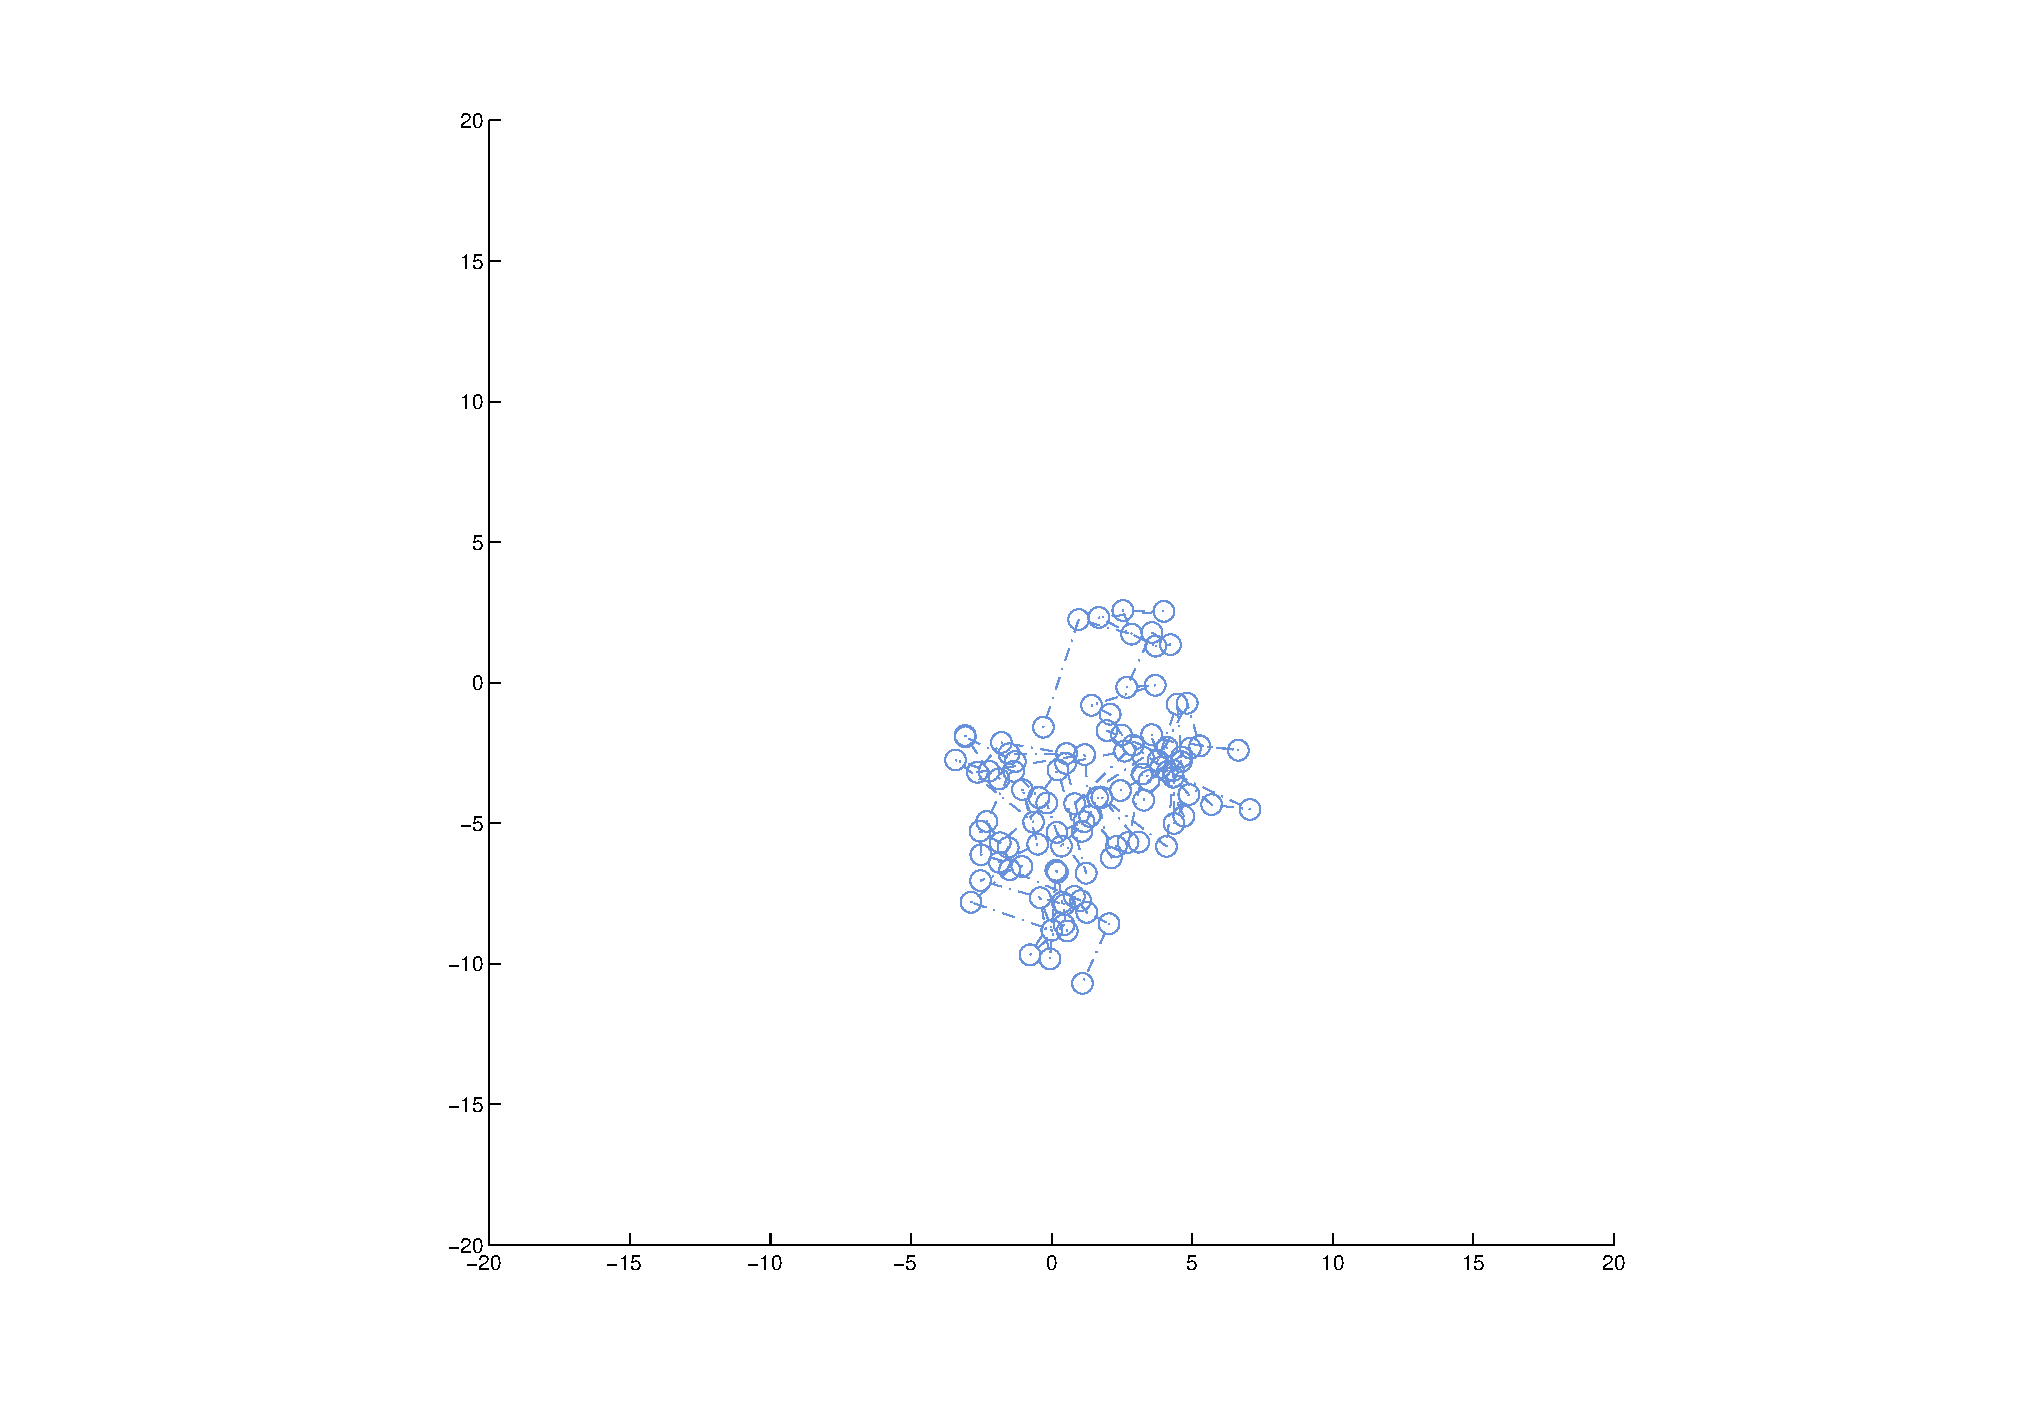
\includegraphics[width=3.2in]{1.eps}
		\caption{initial position}
	\end{minipage}%
	\begin{minipage}[t]{0.5\textwidth}
		\centering
		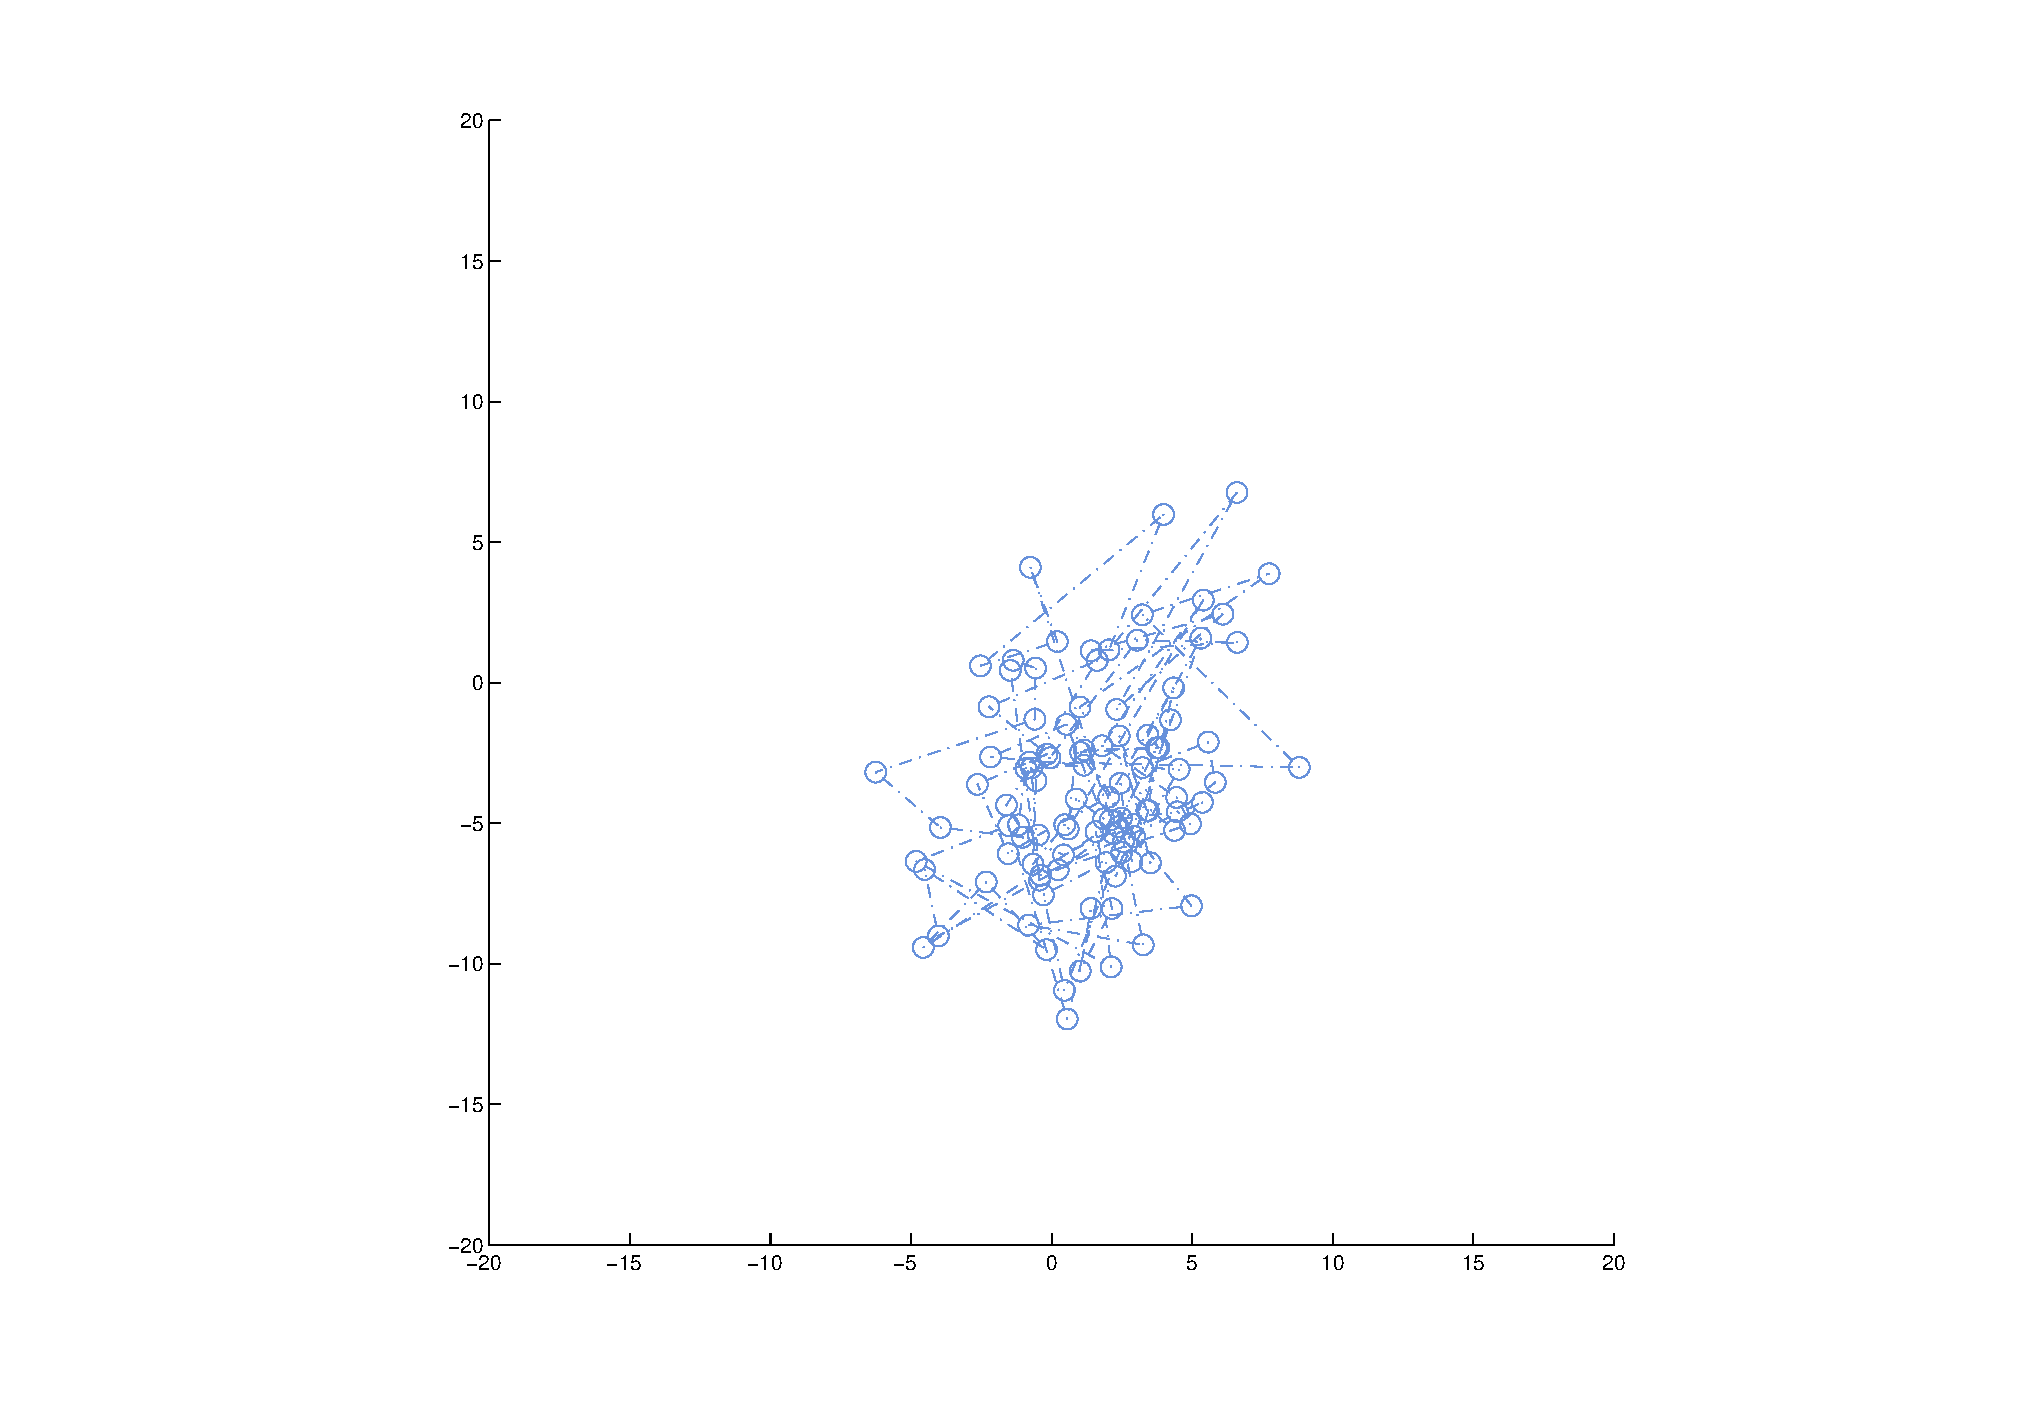
\includegraphics[width=3.2in]{2.eps}
		\caption{final position}
		
	\end{minipage}
\end{figure}
\subsection{Probability distribution function of $\bm{R}$  }
In order to verify that the PDF of $\bm{R}$ is Gaussian,we calculate the 'end to end distance' $\bm{R}$ for each simulation,then we plot it with histogram by coordinate $(x,y,z)$ respectively and compare with the probability
\begin{figure}[H]
	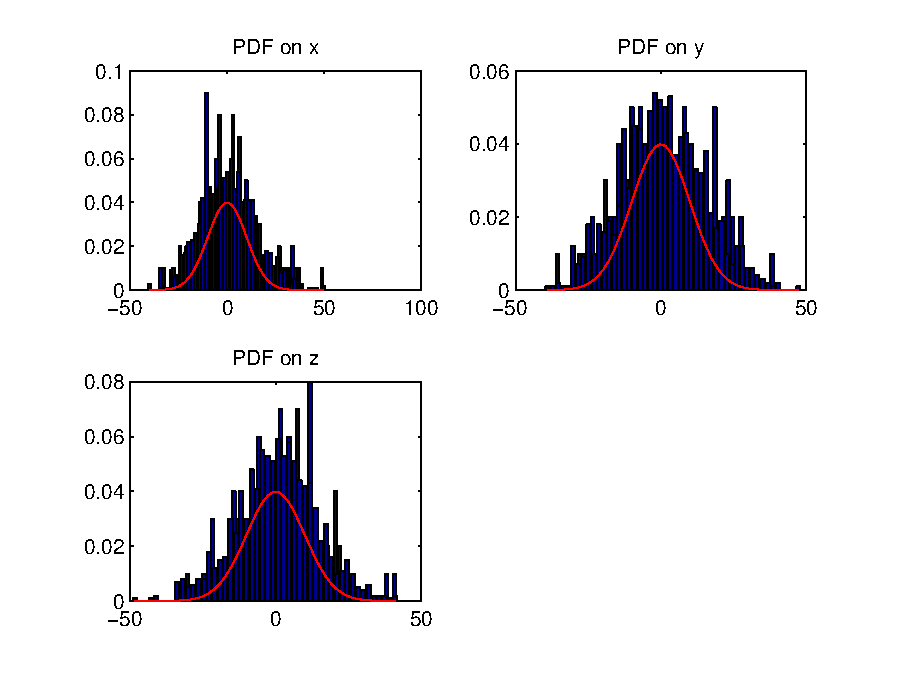
\includegraphics[width=4.2in]{PDF.eps} 
	 
	 \end{figure}
\end{document}